% !TEX root = ../paper.tex

\section{Design}

\improve{Explain basic design}

\improve{sequential, parallel part}

\begin{figure}[htb]
	\centering
	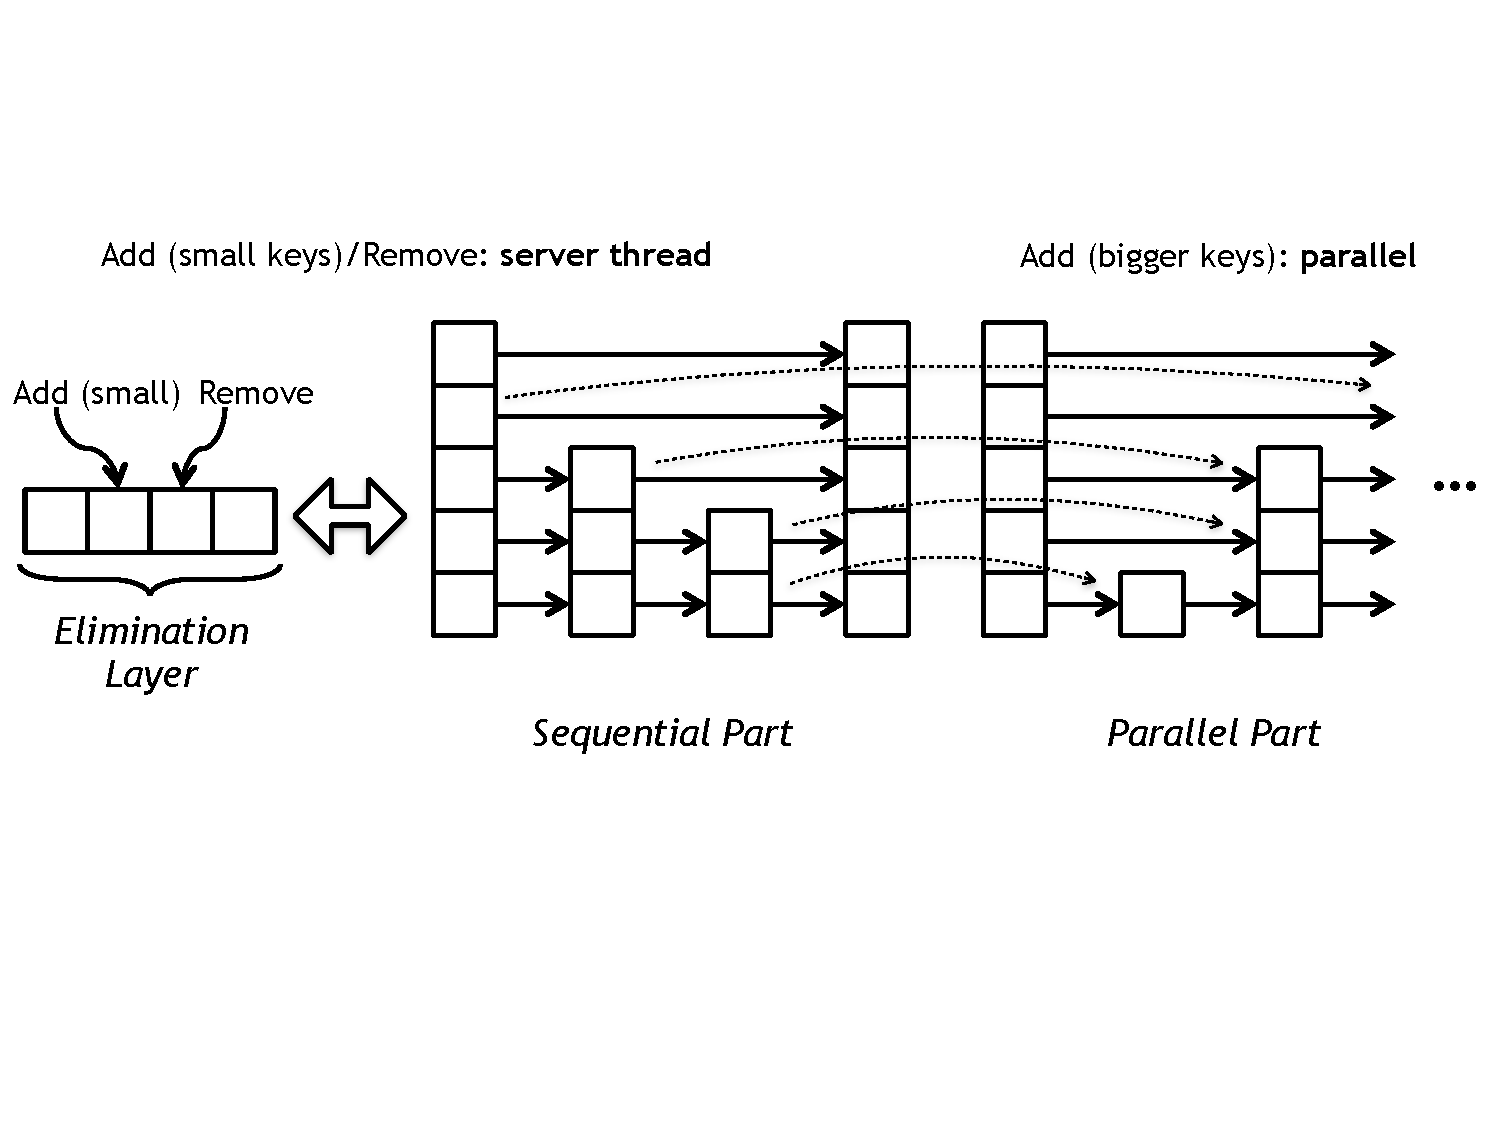
\includegraphics[width=0.9\textwidth]{graphics/pqe.pdf}
	\caption{\cite{calciu_adaptive_2014}}
	\label{fig:pqe}
\end{figure}

\paragraph{Add() Operation}

\texttt{PQ:add()} asdf bla faseel

\paragraph{RemoveMin() Operation}

\subsection{Elimination and Combining}

\subsubsection{Elimination Array Transitions}

\begin{figure}[htb]
	\centering
	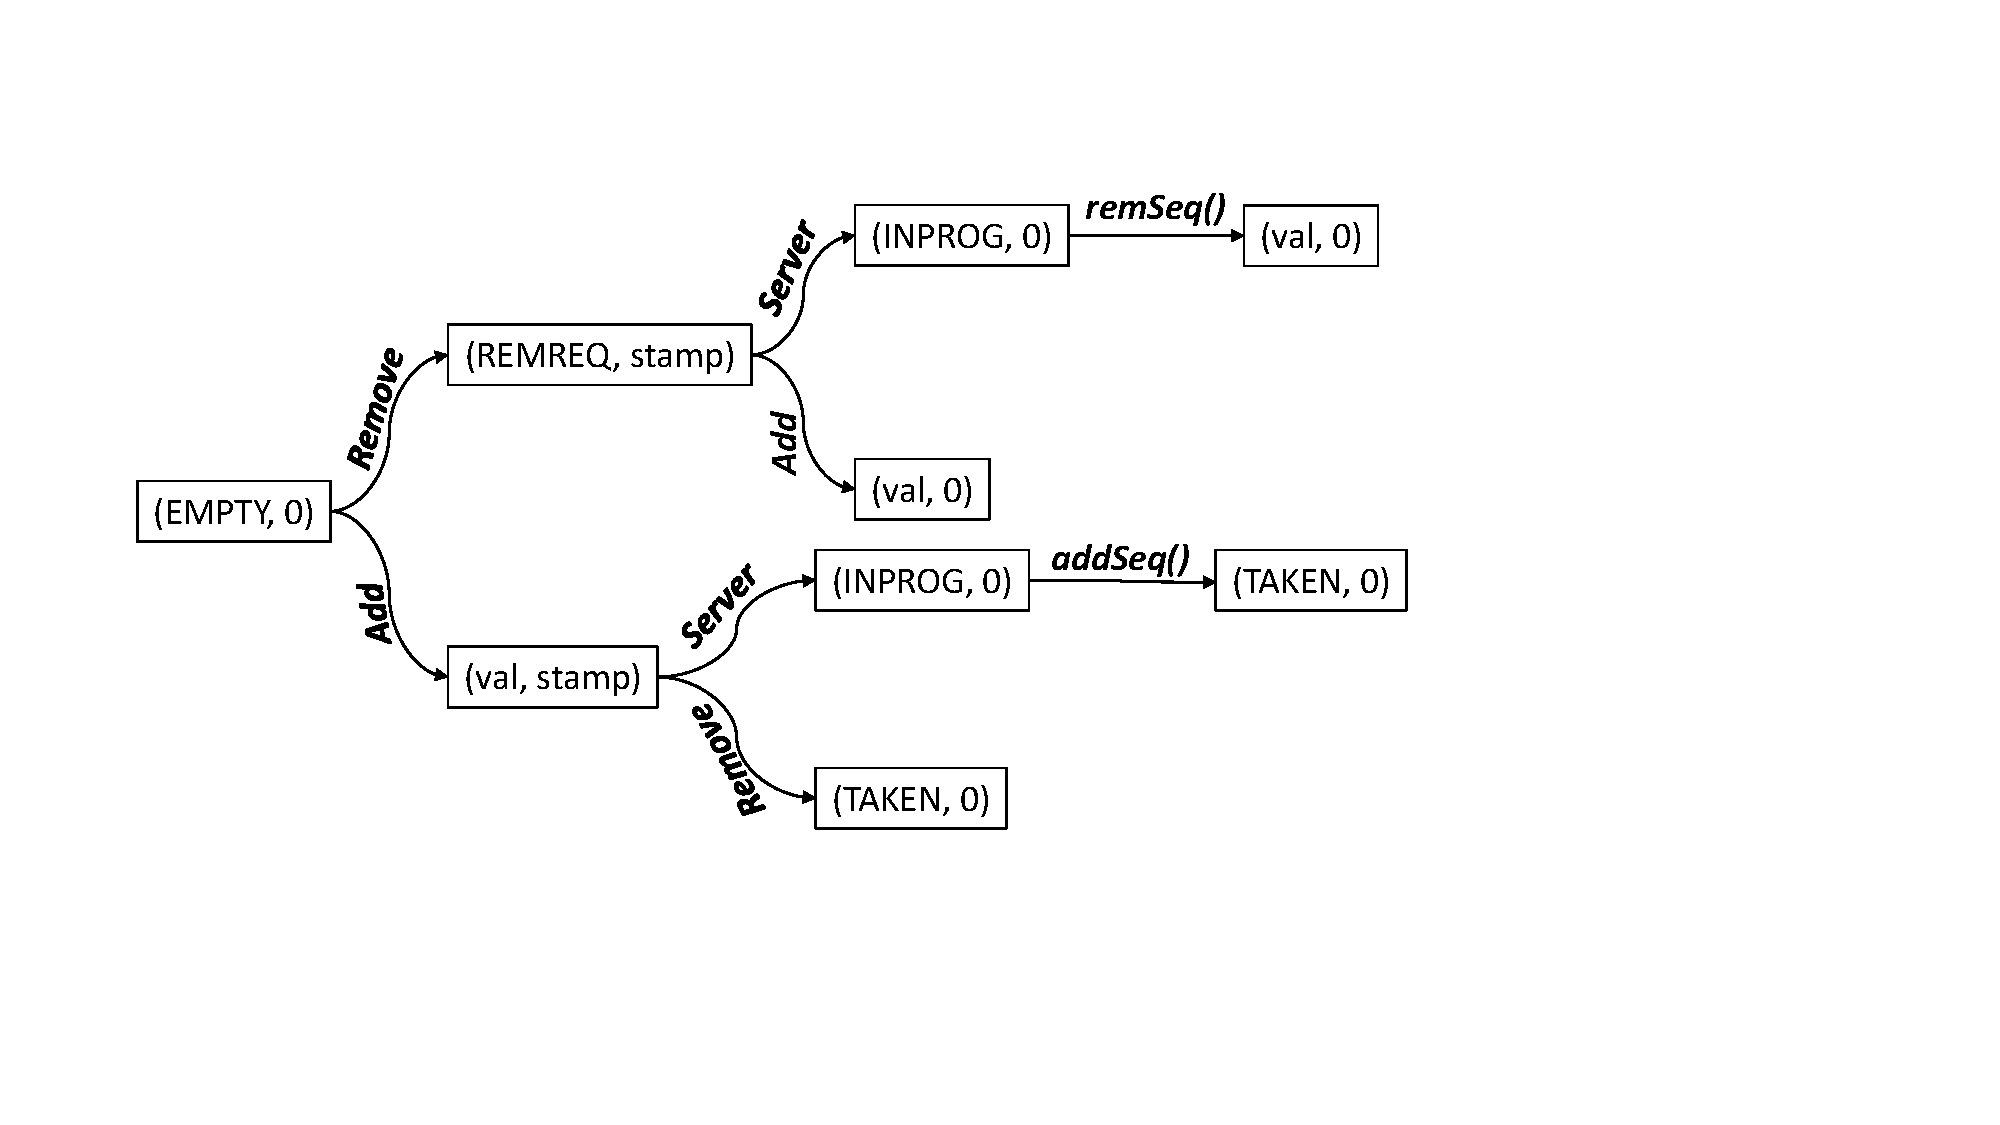
\includegraphics[width=0.9\textwidth]{graphics/combining-state.pdf}
	\caption{\cite{calciu_adaptive_2014}}
	\label{fig:pqe}
\end{figure}

\subsubsection{Server Thread}

\subsection{Skiplist Operations}

\subsubsection{Sequential Part Operations}

\paragraph{addSeq()}

\paragraph{moveHead()}

\paragraph{chopHead()}

\subsubsection{Parallel Part Operations}

\paragraph{addPar()}

\subsection{Hardware Transactions}

\subsubsection{Head-Moving Operations}

\subsubsection{addPar()}
